\section{ИССЛЕДОВАНИЕ РАБОТЫ ПАРАЛЛЕЛЬНОГО РЕГИСТРА}

Микросхема имеет следующие входы:
тактовый С,
информационные D0 – D3,
управления загрузкой P1 и P2,
сброса R и считывания выходных данных Е1 и Е2.
Операция загрузки происходит синхронно с фронтом тактового импульса на входе С,
если на входах Р1 и Р2 одновременно присутствует сигнал логического 0.

Хранящийся в регистре цифровой код может быть считан c выходов
Q0 – Q3, если на входы управления считыванием Е1 и Е2 одновременно
подан сигнал логического 0. Выходными каскадами данной микросхемы
являются буферные логические элементы с тремя логическими
состояниями, Если хотя бы на одном из входов присутствует сигнал
логической 1, выходы находятся в высокоимпедансном состоянии (Z-состояние) и считывание информации запрещено. Это позволяет
подключать выходы регистра непосредственно к шине данных
микропроцессорных устройств

\begin{figure}[H]
	\centering
	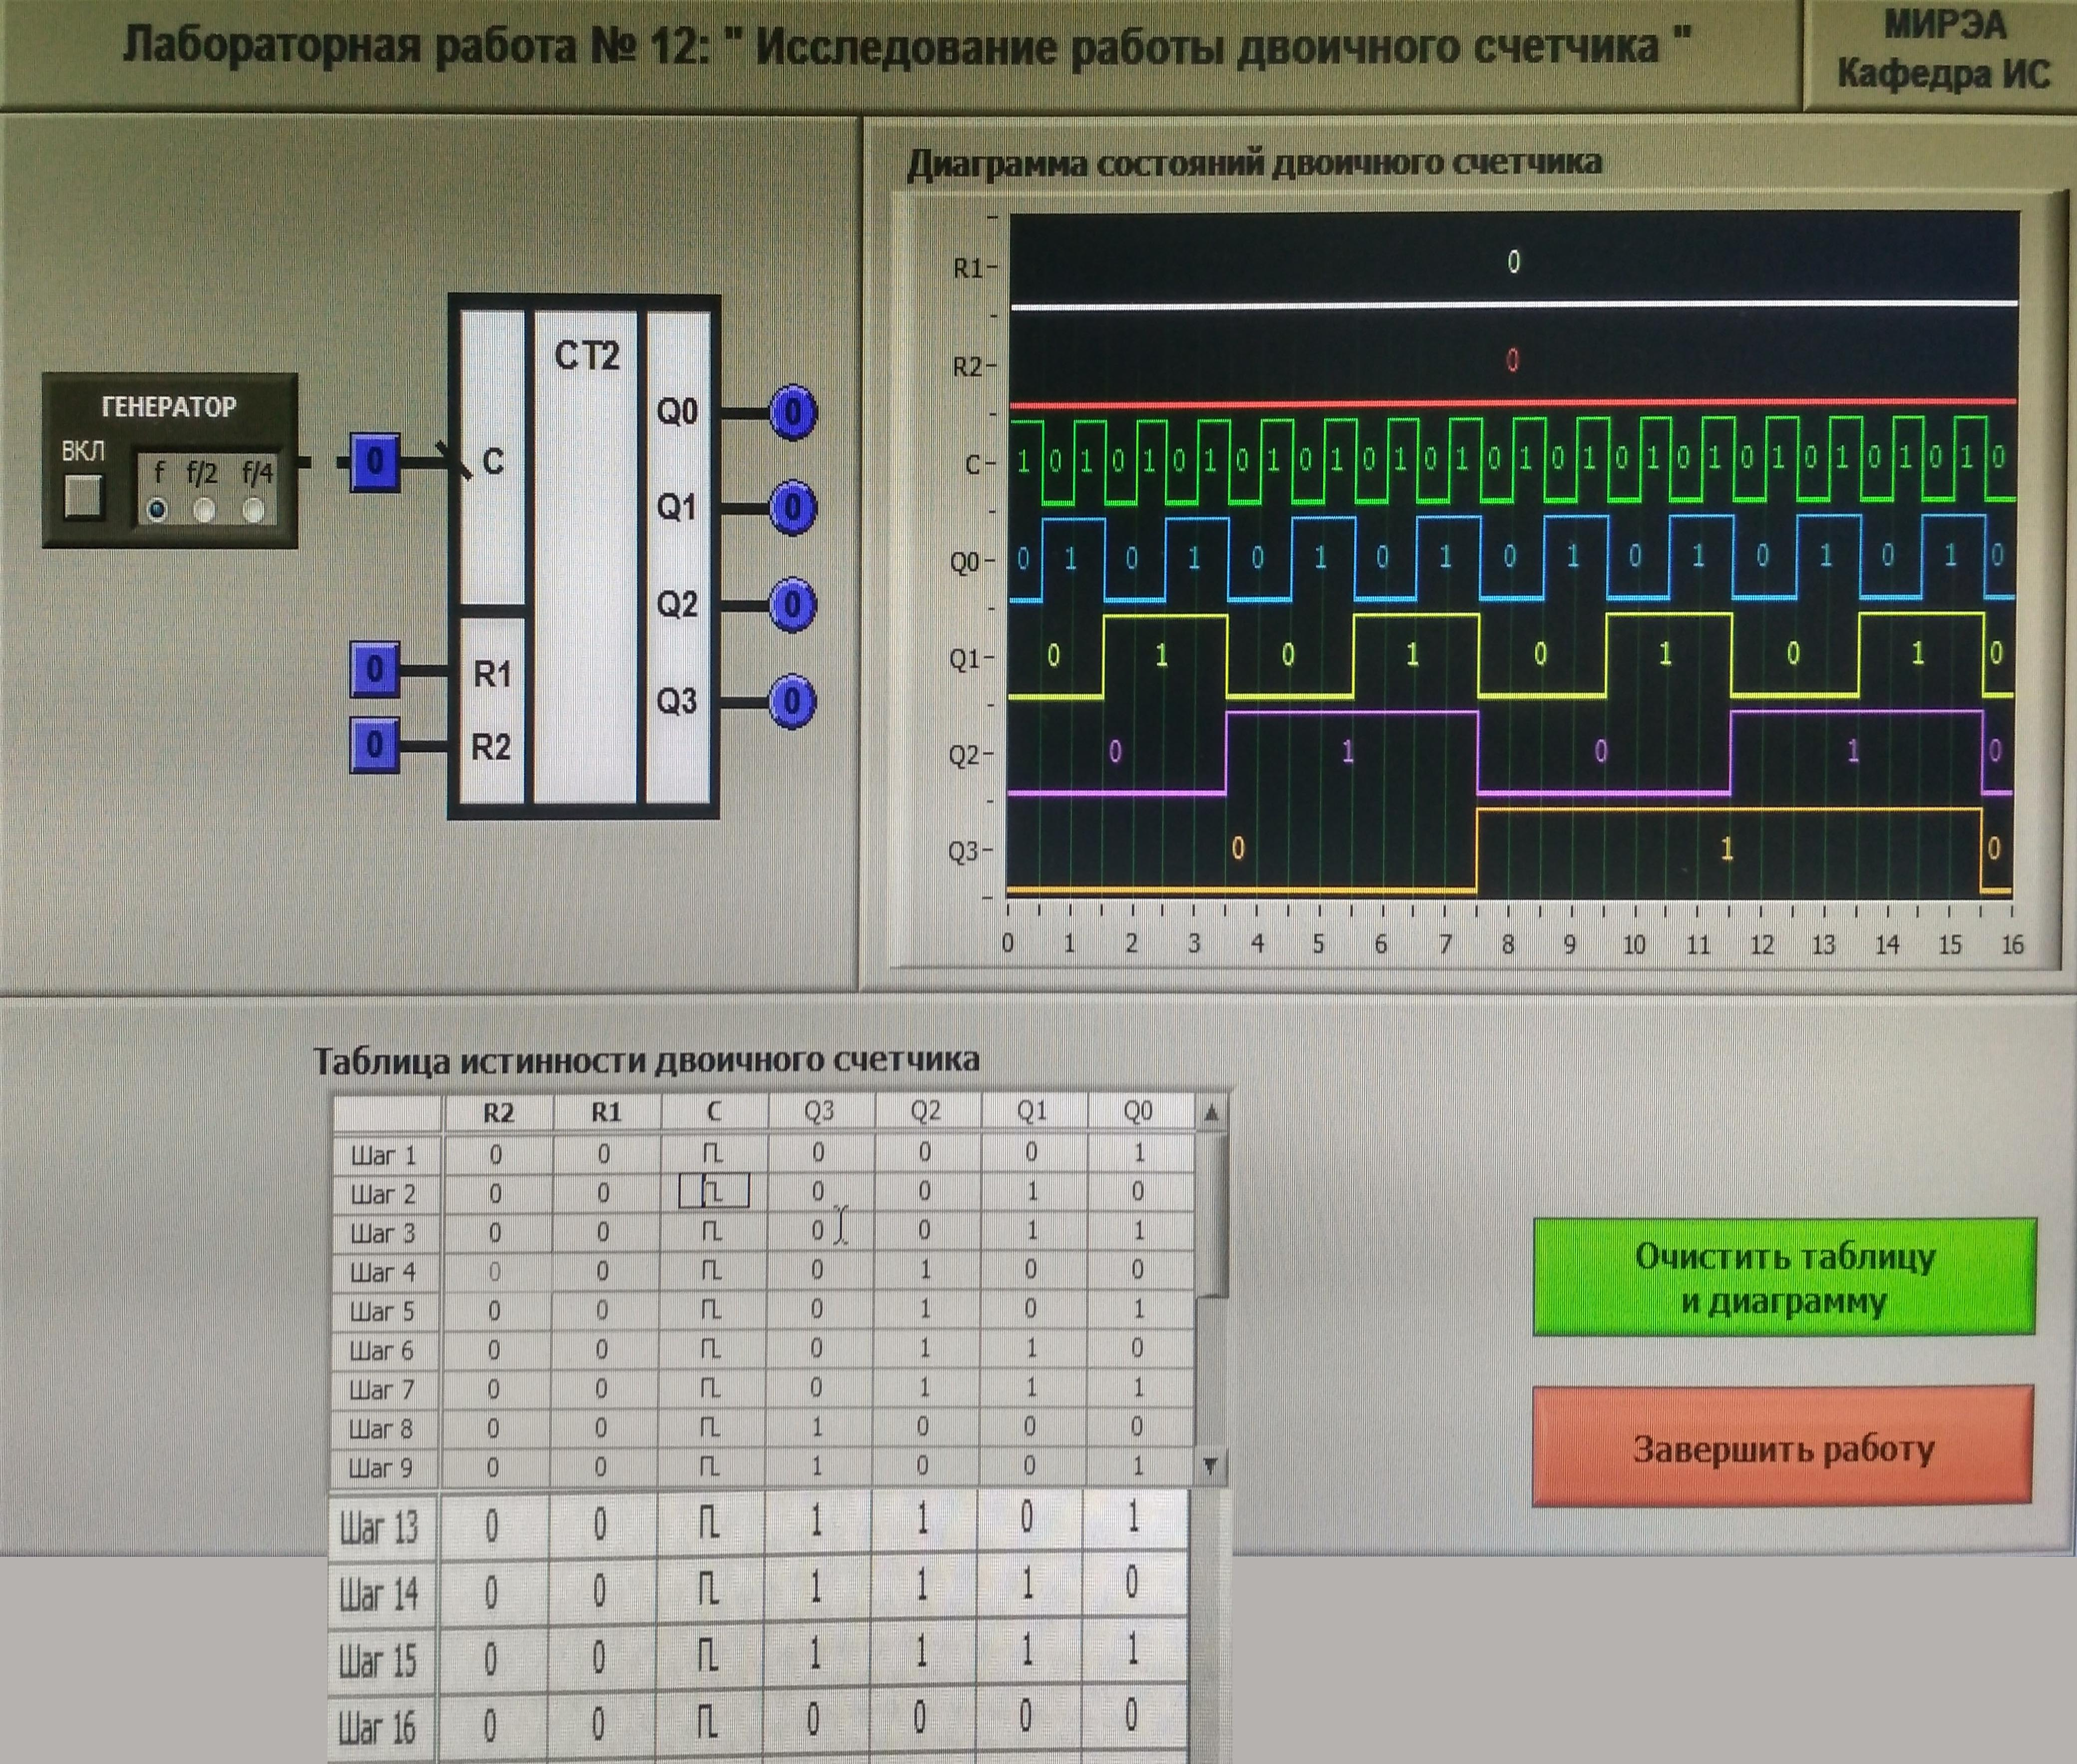
\includegraphics[width=0.95\linewidth]{imgs/10/1.jpg}
	\caption{Режим параллельной загрузки и хранения}
	\label{fig:10_1}
\end{figure}

\begin{figure}[H]
	\centering
	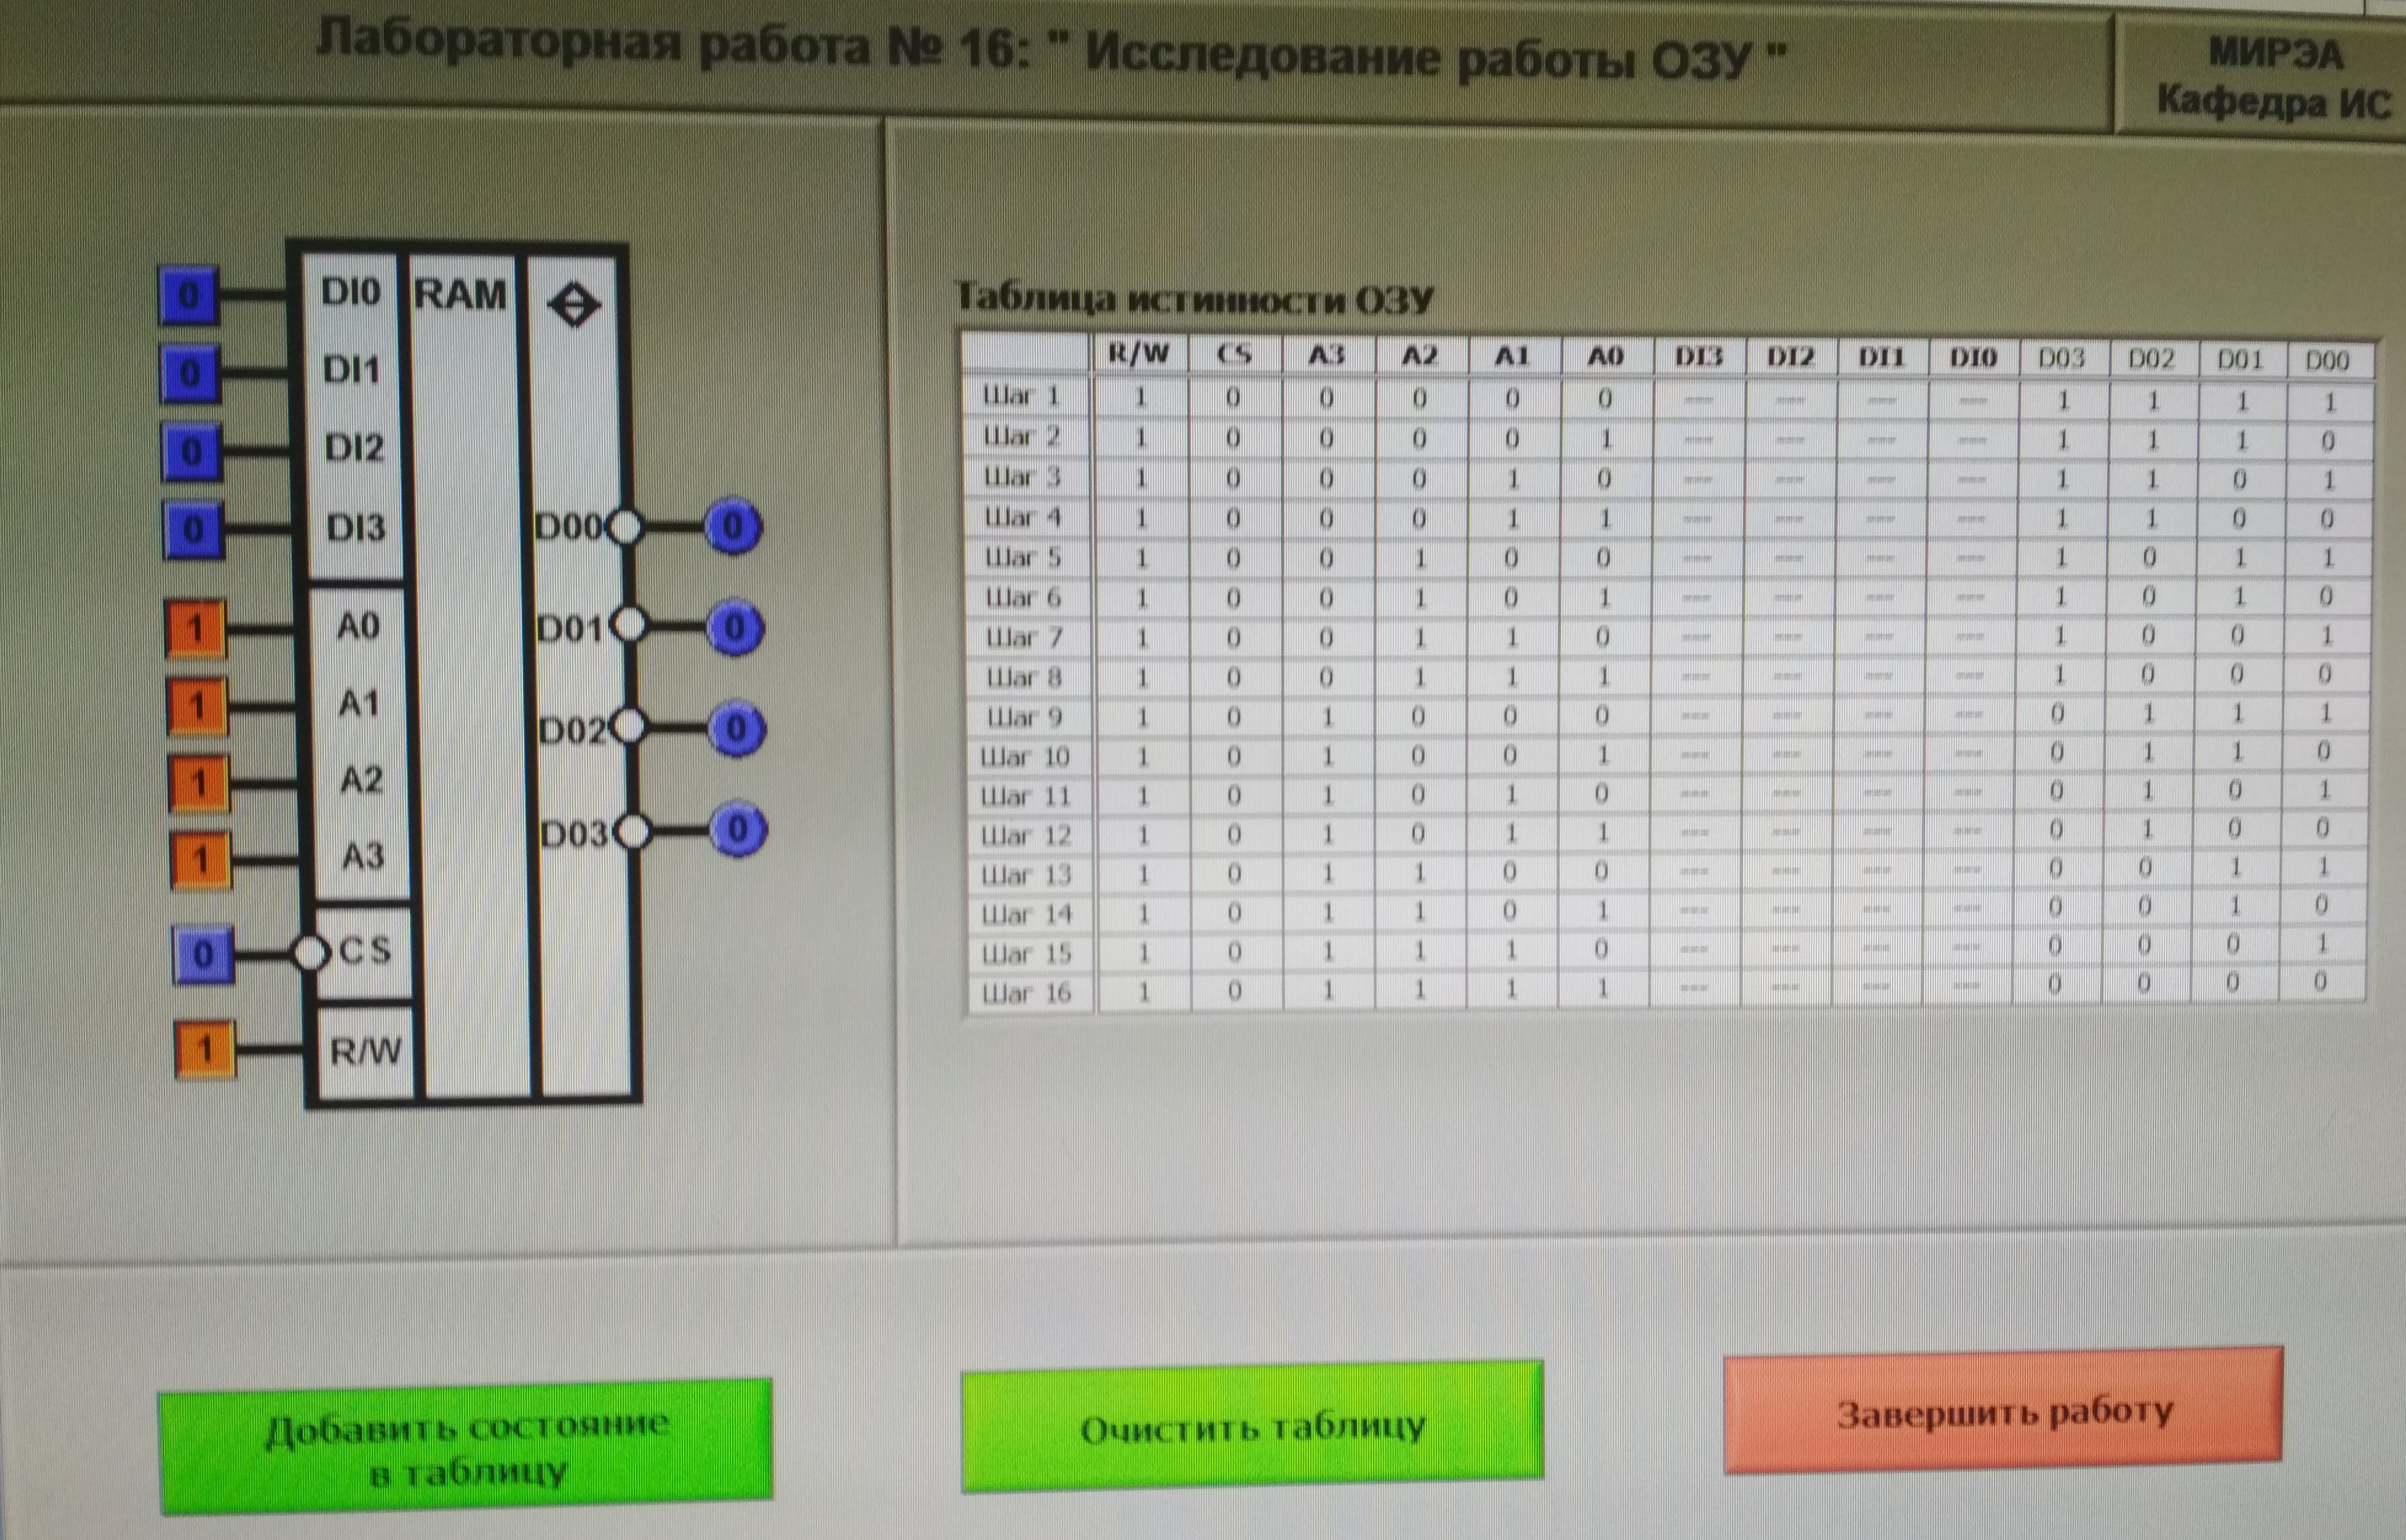
\includegraphics[width=0.95\linewidth]{imgs/10/2.jpg}
	\caption{Режим параллельной загрузки и хранения}
	\label{fig:10_2}
\end{figure}


% Шифратор является приоритетным, вход X6 имеет больший приоритет, чем X3

\begin{figure}[H]
	\centering
	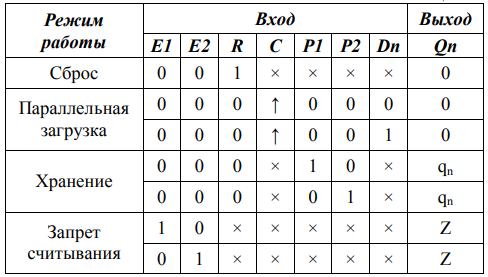
\includegraphics[width=0.95\linewidth]{imgs/10/10_tab}
	\caption{Режим работы регистра}
	\label{fig:10_tab}
\end{figure}

Элемент SN74173N - TTL

Характеристики:

\begin{figure}[H]
	\centering
	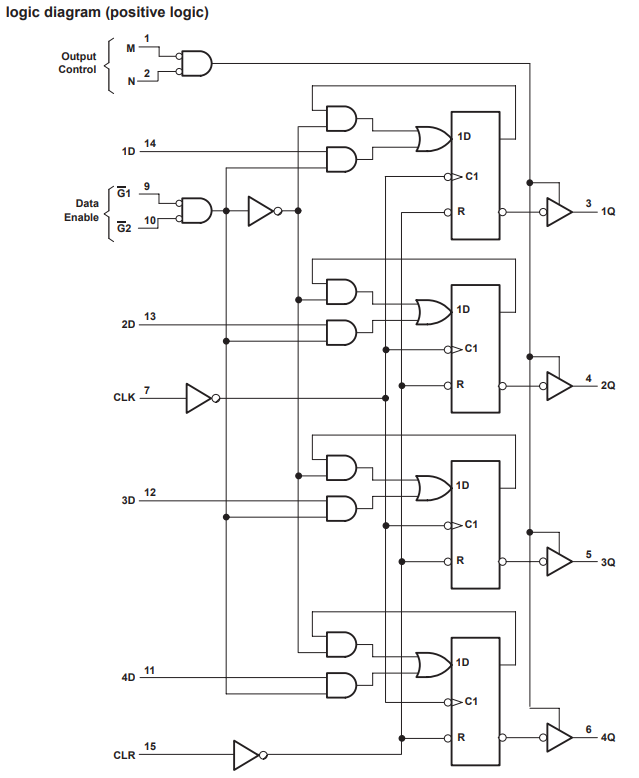
\includegraphics[width=0.95\linewidth]{imgs/10/10_sh}
	\caption{Схема}
	\label{fig:10_sh}
\end{figure}

\begin{figure}[H]
	\centering
	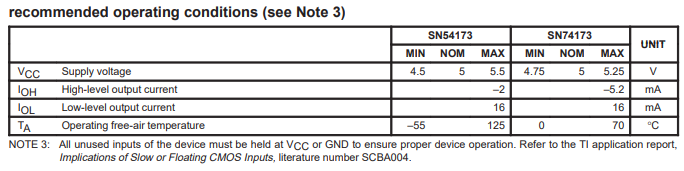
\includegraphics[width=0.95\linewidth]{imgs/10/10_rec}
	\caption{Рекомендуемые рабочие параметры}
	\label{fig:10_rec}
\end{figure}

\begin{figure}[H]
	\centering
	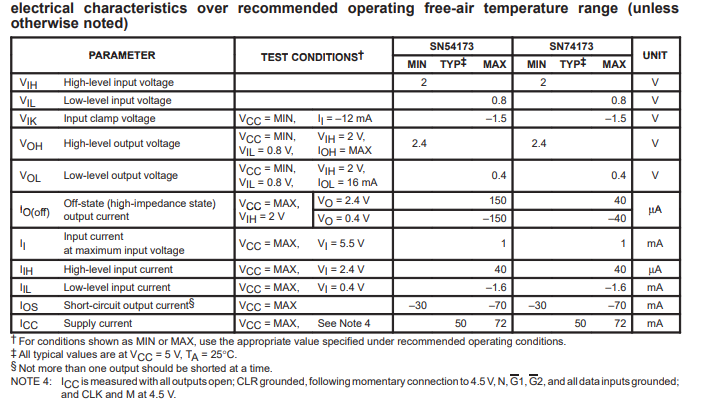
\includegraphics[width=0.95\linewidth]{imgs/10/10_ch}
	\caption{Электрические характеристики}
	\label{fig:10_ch}
\end{figure}

\begin{figure}[H]
	\centering
	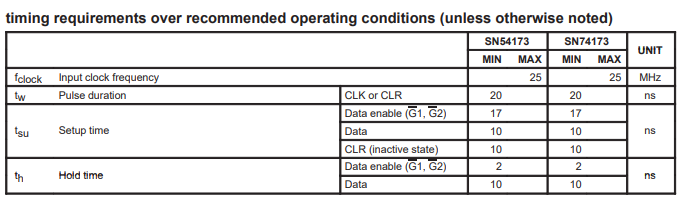
\includegraphics[width=0.95\linewidth]{imgs/10/10_timing}
	\caption{Временные характеристики}
	\label{fig:10_timing}
\end{figure}

\begin{figure}[H]
	\centering
	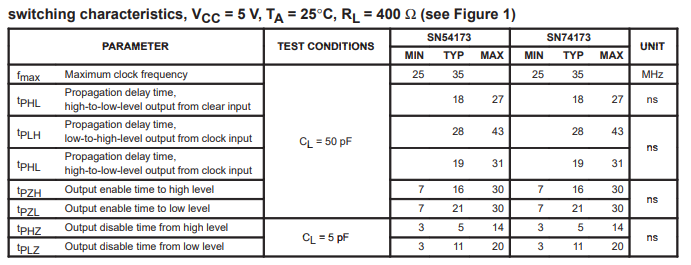
\includegraphics[width=0.95\linewidth]{imgs/10/10_switch}
	\caption{Коммутационные характеристики}
	\label{fig:10_switch}
\end{figure}